 \documentclass{report}
 
\usepackage[utf8]{inputenc} 
\usepackage[T1]{fontenc}      
\usepackage[top=2.0cm, bottom=3cm, left=3.0cm, right=3.0cm]{geometry}
\usepackage{graphicx}
\usepackage{wrapfig}
\usepackage{amsmath,esint }
\usepackage{amssymb}
\usepackage{esvect}
\graphicspath{{figures/}{../figures}}

\newcommand*\dif{\mathop{}\!\mathrm{d}}
\newcommand*\diver{\mathop{}\!\mathrm{div}}
\newcommand*\grad{\mathop{}\!\mathrm{grad}}

\begin{document}

\section*{Approche ontologique du champ magnétique $\bullet\bullet\circ$}

On considère un fil électrique de section $\Sigma$ dirigé suivant l'axe $x$. Il est constitué d'atomes séparés d'une distance $a$, de charge $+e$  et d'autant d'électrons de conduction de charge $-e$ ; on suppose que atomes et électrons sont confondus sur l'axe $x$ et uniformément répartis à travers la section $\Sigma$. On impose un courant $I$ dans le fil, les électrons se déplacent alors avec une vitesse $\vec{v'}=-v'\vec{e_{x}}$ uniforme le long du fil.

Une particule de charge $q$ se déplace à la vitesse $\vec{v}=v\vec{e_{x}}$ à l'extérieur du fil à une distance $r>a$ de l'axe $x$.

\begin{figure}[h!]
\centering
		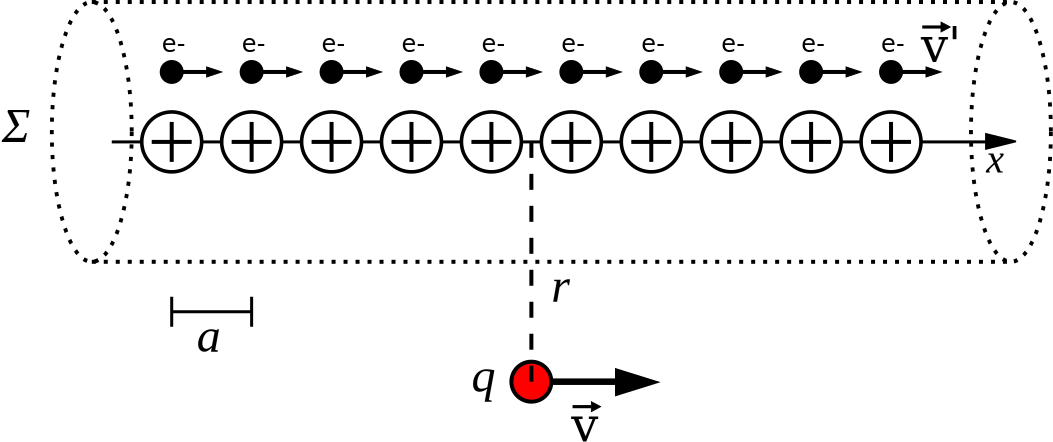
\includegraphics[scale=0.25]{cable.pdf}
\end{figure}

On s'intéresse aux forces électromagnétiques exercées par les charges du fil sur la particule de charge $q$ par deux approches différentes.

\subsubsection*{Approche en mécanique classique}

\begin{itemize}
	\item[$\clubsuit$] Quelle est la densité de charge $\rho_{+}$ (respectivement $\rho_{-}$) due aux atomes (resp. aux électrons) dans le fil ? En déduire le champ électrique $\vec{E}$ créé par cette distribution de charge pour $r>a$.
	
	\item[$\clubsuit$] Quelle est la densité de courant $\vec{j}$ dans le fil ? Exprimer la vitesse $\vec{v'}$ des électrons de conduction en fonction de $I$. En déduire le champ magnétique $\vec{B}$ créé par ce courant en fonction de $v'$ et des autres données de l'énoncé.
	\item[$\clubsuit$] Exprimer la force totale s'exerçant alors sur la charge $+q$, en fonction de $q$, $v$, $v'$, $a$, $r$ et de constantes fondamentales. Quels sont les contributions des forces électriques et magnétiques sur cette particule ?
	\item[$\clubsuit$] Que devient cette force dans le référentiel en mouvement de la charge $+q$ ? En quoi est-ce une contradiction ?
\end{itemize}

\subsubsection*{Approche en mécanique relativiste}

La théorie de la relativité restreinte permet de lever cette contradiction, en affirmant que tout objet se déplaçant relativement par rapport à un autre voit sa longueur contractée dans le sens du déplacement. Ainsi, Einstein a démontré en 1905 qu'un objet à la vitesse $v$ par rapport à un autre objet, voit la longueur de ce dernier contractée d'un facteur $\gamma(v)=1/\sqrt{1-v^{2}/c^{2}}$ (où $c$ est la vitesse de la lumière). Dans son référentiel, la charge $q$ voit donc la densité de charge des atomes $\rho_+$ et des électrons $\rho_-$ augmenter, mais pas dans les mêmes proportions. 
	\begin{itemize}
		\item[$\clubsuit$] Que deviennent les densités de charge $\rho_{+}$ et $\rho_{-}$ dans le référentiel de la particule $+q$ ? %On admettra que les électrons se déplacent à la vitesse $v'-v$ dans le référentiel de $+q$. 
		\item[$\clubsuit$] Déterminer le champ électrique créé par cette nouvelle distribution de charges en fonction de $v$, $v'$, $a$, $r$ et de constantes fondamentales. On supposera que $v'\ll v\ll c$.
		\item[$\clubsuit$] Quelle est la force électrique s'exerçant sur la particule $+q$ ? 
		\item[$\clubsuit$] Comparer avec le résultat trouvé en approche classique (non relativiste). Que peut-on en dire sur la nature du champ magnétique ?
	\end{itemize}
			
\textit{N.B.} : On rappelle que la vitesse de la lumière $c$ est définie comme $c^{2}=1/\epsilon_{0}\mu_{0}$, où $\epsilon_{0}$ et $\mu_{0}$ sont respectivement la permittivité électrique et la perméabilité magnétique du vide.

\newpage

\section*{\textit{Correction Approche ontologique du champ magnétique}}

\subsubsection*{Approche en mécanique classique}

\begin{itemize}
	\item[$\clubsuit$] Dans une volume $a\Sigma$, on a une charge $+e$ et une charge $-e$, comme celle-ci sont réparties uniformément. Les densités de charges sont donc respectivement $\rho_+=e/(a\Sigma)$ et $\rho_-=-e/(a\Sigma)$.
	\item[$\clubsuit$] Par définition, $\vec{j}=\rho\vec{v}$. Comme seuls les électrons ont une vitesse non nulle, $\vec{j}=\rho_-\vec{v'}=ev'/(a\Sigma)\vec{e}_x$. Et donc $I=\oiint_\Sigma\dif\vec{S}\vec{j}=ev'/a$.
	\item[$\clubsuit$] $\rho_{tot}=\rho_++\rho_-=0$ donc $\vec{E}=0$.
	\item[$\clubsuit$] Avec le théorème d'Ampère appliqué uniquement en dehors du fil, on trouve :
	\begin{align*}
		\vec{B}=\frac{\mu_0I}{2\pi r}\vec{e_\theta}
	\end{align*}
	(résultat classique d'un fil parcouru par un courant $I$)
	La force qui s'exerce sur la charge $q$ est donc :
	\begin{align*}
		\vec{F}=-\frac{qv\mu_0I}{2\pi r}\vec{e_r}
	\end{align*}
\end{itemize}

\subsubsection*{Approche en mécanique relativiste}

	\begin{itemize}
	
		\item[$\clubsuit$] Ainsi, en se déplaçant à la vitesse $\vec{v}$, la charge $+q$ voit dans son référentiel la distance entre atomes réduite d'un facteur $\gamma_{+}=1/\sqrt{1-v^{2}/c^{2}}$ et la distance entre électrons de conduction d'un facteur $\gamma_{-}=1/\sqrt{1-(v-v')^{2}/c^{2}}$. 
		On trouve donc que :
		\begin{align*}
			\rho_+=\frac{e}{a\Sigma}\sqrt{1-v^{2}/c^{2}}
		\end{align*}
		\begin{align*}
			\rho_-=\frac{e}{a\Sigma}\sqrt{1-(v+v')^{2}/c^{2}}
		\end{align*}		
		Attention, l'hypothèse que la vitesse relative des électrons par rapport à la charge $q$ est $v'+v$ est une approximation. En mécanique relativiste, la vitesse relative serait :
		\begin{equation}
			v_{e_-/q}=\frac{v'-v}{1-\frac{vv'}{c^2}}
		\end{equation}
		
	\item[$\clubsuit$] On trouve facilement avec le théorème de Gauss que :
	\begin{align*}
		\vec{E}=\frac{\Sigma(\rho_++\rho_-)}{2\pi r\varepsilon_0}
	\end{align*}
	
	 En développant à l'ordre 2, on trouve :
	\begin{align*}
		\rho_++\rho_-\approx -\frac{e}{a\Sigma}\frac{vv'}{c^2}
	\end{align*}
	On trouve alors que :
	\begin{align*}
		\vec{E}=-\frac{e vv'}{2\pi r a\varepsilon_0 c^2}\vec{e_r}=-\frac{I\mu_0 v}{2\pi r}\vec{e_r}
	\end{align*}
	
	\item[$\clubsuit$]
	La force de Lorentz associée est donc :
	\begin{align*}
		\vec{F}=-\frac{qe vv'}{2\pi r a\varepsilon_0 c^2}\vec{e_r}=-\frac{qI\mu_0 v}{2\pi r}\vec{e_r}
	\end{align*}
	
	Cette expression est identique à celle trouvée par le calcul du champ magnétique en mécanique classique. Le champ magnétique est-il est une approximation à l'ordre 2 de la force de Coulomb ? 
	\end{itemize}

\newpage

\section*{Câble coaxial $\bullet\bullet\circ$}

On considère un câble coaxial constitué de deux conducteurs cylindriques de même axe, séparés par du vide, de rayon $a$ (l'âme) et $b$ (la gaine), avec $a<b$, et d'épaisseur négligeable. Le conducteur central (de rayon $a$) a une charge surfacique $\sigma_a$ répartie uniformément et est traversé par une densité surfacique de courant $\vec{j_{s,a}}$, répartie aussi uniformément sur l'âme. La longueur du câble est $L$, très grande devant les rayons $a$ et $b$.  

\begin{figure}[h!]
\centering
		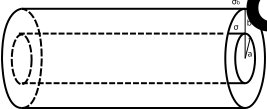
\includegraphics[scale=1]{em2.pdf}
\end{figure}

On cherche à connaitre la capacité et l'inductance linéique du câble coaxial, pour comprendre la propagation des ondes électromagnétiques à l'intérieur. 

\begin{itemize}

	\item[$\blacksquare$] Exprimer le courant $I$ circulant dans l'âme et sa charge totale $Q$ en fonction de $\vec{j_{s,a}}$ et $\sigma_a$. En déduire la charge et l'intensité surfacique de la gaine, $\sigma_b$ et $\vec{j_{s,b}}$, sachant que, sur toute la longueur du câble, le courant total à travers le câble est nul et qu'il est neutre électriquement.
	
	\item[$\blacksquare$] Déterminer le champ électrique en tout point.

	\item[$\blacksquare$] En déduire la capacité $c$ par unité de longueur de câble. 
	
	\item[$\blacksquare$]	 Déterminer le champ magnétique en tout point. 
	
	\item[$\blacksquare$] On définit l'inductance $L$ d'un circuit délimitant une surface $S$, parcouru par un courant $I$ comme  comme le rapport du flux du champ magnétique à travers $S$ avec le courant $I$ :
	\begin{align*}
		\Phi_B=\oiint_S \dif \vec{S}\cdot\vec{B}=LI
	\end{align*}
En choisissant soigneusement une surface $S$, déterminer l'inductance linéique $l$. 

	\item[$\blacksquare$] Que vaut le produit le produit $l\times c$ ? A quoi correspond cette grandeur ?
	
\end{itemize}

\newpage

\section*{\textit{Correction Câble coaxial}}

\begin{itemize}

	\item[$\heartsuit$] Le courant circulant dans l'âme est $I=2\pi a j_{s,a}$. De même, la charge totale est $Q=2\pi a l \sigma_a$. On a forcément $I=2\pi b j_{s,b}$. De même, la charge totale est $Q=2\pi b l \sigma_b$ par conservation de la charge et du courant. 
	
	\item[$\heartsuit$] Les symétries et les invariances donnent $\vec{E}=E(r)\vec{e_r}$. Avec le théorème de Gauss appliqué sur un cylindre de rayon $r$, on obtient :
	\begin{align*}
	\left\lbrace
	\begin{array}{ccc}
	r<a & : & \vec{E}=\vec{0} \\
	a<r<b & : & \vec{E} = \frac{\sigma_a a}{\varepsilon_0 r}\vec{e_r} \\
	r>b & : & \vec{E}=\vec{0}
	\end{array}\right.
\end{align*}

	\item[$\heartsuit$] On en déduit le potentiel entre les deux conducteurs :
	\begin{align*}
		V=\frac{\sigma_aa}{\varepsilon_0}\ln\left(\frac{b}{a} \right) =\frac{Q}{2\pi l\varepsilon_0}\ln\left(\frac{b}{a} \right)
	\end{align*}
La capacité par unité de longueur est donc :
\begin{align*}
	c = \frac{2\pi\varepsilon_0}{\ln\left(\frac{b}{a} \right)}
\end{align*}

	\item[$\heartsuit$] Les symétries et les invariances donnent $\vec{B}=B(r)\vec{e_\theta}$. Avec le théorème de d'Ampère appliqué sur un cercle de rayon $r$, on obtient :
	\begin{align*}
	\left\lbrace
	\begin{array}{ccc}
	r<a & : & \vec{B}=\vec{0} \\
	a<r<b & : & \vec{B} = \frac{\mu_0j_{s,a} a}{r}\vec{e_\theta} \\
	r>b & : & \vec{B}=\vec{0}
	\end{array}\right.
\end{align*}

	\item[$\heartsuit$] Le flux du champ $\vec{B}$ se calcule sur la surface rectangulaire comprises entre $a$ et $b$, de longueur $l$ avec $\vec{e_\theta}$ comme vecteur normal. On trouve alors :
	\begin{align*}
		\Phi_B=\frac{L\mu_0I}{2\pi}\ln\left(\frac{b}{a} \right)
	\end{align*}
	On a donc :
	\begin{align*}
		l=\frac{\mu_0}{2\pi}\ln\left(\frac{b}{a} \right)
	\end{align*}

	\item[$\heartsuit$] On trouve que $l\times c=\varepsilon_0\mu_0=\frac{1}{c^2}$. Cela correspond à l'inverse du carré de la vitesse de la lumière, qui est la vitesse de propagation dans le câble coaxial.
	
\end{itemize}

\newpage

\section*{Champ magnétique entre deux nappes de courant $\bullet\circ\circ$}

Deux nappes de courant identiques de très grande surface $S = L_x\times L_y$, d’épaisseur $e$, sont parallèles entre elles et séparées d’une longueur $2a$ par un matériau isolant. Elles sont parcourues par un courant permanent de vecteur densité $J\vec{e}_x$ pour la nappe supérieure 1 et $-J\vec{e}_x$ pour la nappe inférieure 2. On se place suffisament loin des bords de la nappe pour négliger les effets de bord.

\begin{figure}[h!]
\centering
		\includegraphics[scale=0.7]{nappe_courant.png}
\end{figure}

\begin{itemize}
	
	\item[$\clubsuit$] Etudier la dépendance et la direction du champ magnétique à partir des symétries et invariances.
	
	\item[$\clubsuit$] Déterminer rigoureusement le champ magnétique dans tous l'espace, et le représenter sur un graphe.
	
\end{itemize}

On définit l'inductance $L$ d'un circuit délimitant une surface $S$, parcouru par un courant $I$ comme  comme le rapport du flux du champ magnétique à travers $S$ avec le courant $I$ :
	\begin{align*}
		\Phi_B=\oiint_S \dif \vec{S}\cdot\vec{B}=LI
	\end{align*}

\begin{itemize}

	\item[$\clubsuit$] Quelle est la surface délimitée par le circuit formé par les deux nappes ? En déduire l'inductance formée par ce système. 
	
\end{itemize}

\newpage

\section*{Champ magnétique dans un cylindre parcouru par un courant orthoradial $\bullet\bullet\circ$}

On considère un cylindre conducteur de rayon $a$ et de longueur $L\gg a$ selon l'axe $O_z$, dans lequel circule une densité volumique de courant $\vec{j}(r)=j_0\frac{r}{a}\vec{e}_\theta$.

\begin{itemize}

	\item[$\circ$] A l'aide des symétries et invariances, expliciter la dépendance spatiale et la direction du champ magnétique.
	\item[$\circ$] Déterminer l'expression du champ magnétique $\vec{B}(r)$ en fonction de la valeur du champ magnétique en $r=0$.
	\item[$\circ$] Quel est l'expression du champ magnétique $\vec{B}(r)$ si on impose un champ exterieur $\vec{B}_{ext}$ de sorte à ce que  $\vec{B}(r=a)=\vec{0}$ ? Quelle est alors la valeur de $\vec{B}_{ext}$ ?

\end{itemize}

\newpage

\section*{\textit{Correction Champ magnétique dans un cylindre parcouru par un courant orthoradial}}

\begin{itemize}

	\item[$\circ$] Invariance : le champ ne dépend que de $r$. Symétrie : le plan $(\vec{e}_r ;\vec{e}_\theta)$ est plan de symétrie de la distribution de courant donc $\vec{B}$ est suivant $\vec{e}_z$.
	
	\item[$\circ$] On calcule la circulation de $\vec{B}$ sur le contour $\Gamma$ :
	\begin{figure}[h!]
	\centering
		\includegraphics[scale=0.25]{orthoradial.pdf}
	\end{figure}
	\begin{align*}
		\oint_\Gamma d\vec{l}\cdot\vec{B}&=\int_B^Cdz\times B(r)+\int_D^Adz\times B(0) \\
		&=-hB(r)+hB(0)
	\end{align*}	 
	D'après le théorème d'Ampère, pour $r<a$ :
	\begin{align}
		-hB(r)+hB(0)&=\mu_0j_0h\frac{r^2}{2a}
	\end{align}
	Donc :
	\begin{align*}
		B(r) = B(0)-\mu_0j_0\frac{r^2}{2a}
	\end{align*}
	
	Pour $r>a$ :
	\begin{align*}
		B(r) = B(0)-\mu_0j_0\frac{a}{2}
	\end{align*}	

	\begin{figure}[h!]
	\centering
		\includegraphics[scale=0.25]{orthoradial2.pdf}
	\end{figure}
	
	\item[$\circ$] On ajoute un champ magnétique esxtérieur $\vec{B}_{ext}$, nécessairement selon $\vec{e}_z$ :
	\begin{align*}
		B(r) = B(0)-\mu_0j_0\frac{r^2}{2a} + B_{ext}
	\end{align*}
	Si $B(r=a)=0$ alors $B_{ext}=-B(0)+\mu_0j_0\frac{a}{2}$ et alors :
	\begin{align*}
		B(r) = \frac{\mu_0j_0}{2a}\left( a^2-r^2\right) 
	\end{align*}


\end{itemize}

\newpage

\section*{Foudre $\bullet\circ\circ$}

On modélise la foudre par un tube d'air ionisé cylindrique de rayon $a$=1m et de densité de courant $\vec{j}=j_0\frac{r}{a}\vec{e}_z$. Ce sont les électrons de charge $-e$ qui sont supposés porter le courant électrique.

\begin{itemize}

	\item[$\wr$] Relier le courant total $I$ avec $j_0$ et $a$. Sachant que l'intensité d'un éclair peut atteindre 100 kA, quelle est la densité de courant $j_0$ associée ? 

	\item[$\wr$] Etudier la dépendance et la direction du champ magnétique à partir des symétries et invariances.
	
	\item[$\wr$] Déterminer rigoureusement le champ magnétique dans tous l'espace, et le représenter sur un graphe. Estimer la valeur maximale que prend le champ magnétique.
	
	\item[$\wr$] Rappeler l'expression de la force de Lorentz pour un électron de charge $-e$ lorsqu'il est soumis à un champ magnétique extérieur $\vec{B}$. Expliquer succinctement pourquoi le tube d'air ionisé se contracte sur lui-même, se comprimant fortement et générant une grande quantité de chaleur. 

\end{itemize}

\newpage

\section*{\textit{Correction Foudre}}

\begin{itemize}

	\item[$\wr$] L'intensité s'écrit (où $D$ est le disque de rayon $a$) :
	\begin{align*}
		I &= \oiint_D d\vec{S}\cdot\vec{j} \\
		& = 2\pi j_0\int_0^a \frac{r^2}{a}dr \\
		& = \frac{2}{3}j_0a^2
	\end{align*}
	
	On trouve donc $j_0\simeq50$kA.m$^{-2}$.

	\item[$\wr$] On trouve que $\vec{B}=B(r)\vec{e}_\theta$.
	
	\item[$\wr$] Théorème d'Ampère pour $r<a$ :
	\begin{align*}
	 	& 2\pi\times B(r)=2\pi\mu_0j_0\frac{r^3}{3a} \\
	 	&\Rightarrow B(r) = \mu_0j_0\frac{r^2}{3a}
	\end{align*}
	
	Théorème d'Ampère pour $r>a$ :
	\begin{align*}
	 	& 2\pi\times B(r)=2\pi\mu_0j_0\frac{a^2}{3} \\
	 	&\Rightarrow B(r) = \mu_0j_0\frac{a^2}{3r}
	\end{align*}
	
	\begin{figure}[h!]
\centering
		\includegraphics[scale=0.3]{foudre.pdf}
\end{figure}
	
	\item[$\wr$] Force de Lorentz sur un électron : 
	\begin{align*}
		\vec{f} = -e\vec{E}-e\vec{v}\wedge\vec{B}
	\end{align*}
	
	Ici, $\vec{E}=\vec{0}$ et si $j_0>0$ alors $\vec{v}$ est dirigé suivant $-\vec{e}_z$ et $\vec{B}$ est dirigé suivant $+\vec{e}_\theta$.
	On a donc $\vec{f}$ dirigé suivant $-(-\vec{e}_z)\wedge\vec{e}_\theta=-\vec{e}_r$. Les électrons sont donc attirés vers l'intérieur de l'éclair, se compriement et s'échauffent (faisant de la lumière et du bruit).

\end{itemize}

\end{document}
